\documentclass[letterpaper]{article}
\usepackage[top=3cm,bottom=3cm,left=3cm,right=3cm,marginparwidth=1.75cm]{geometry}
%\usepackage{jheppub}  
\usepackage{listings}
\usepackage{xcolor}
\usepackage{multirow}
%\usepackage{natbib}
\usepackage{dcolumn}
%% Language and font encodings
\usepackage[english]{babel}
\usepackage[utf8x]{inputenc}
\usepackage[T1]{fontenc}
\usepackage{palatino}
\pagestyle{empty} 
%% Sets page size and margins


%% Useful packages
\usepackage{amsmath}
\usepackage{mathrsfs}
\usepackage{amssymb}
\usepackage{afterpage}
\usepackage{graphicx, subcaption}
\usepackage[colorinlistoftodos]{todonotes}
\usepackage[colorlinks=true, linkcolor=blue, citecolor=blue]{hyperref}
\usepackage{aas_macros}

\graphicspath{{./fig/}}

\newcommand{\beq}{\begin{equation}}  
\newcommand{\eeq}{\end{equation}}  
\newcommand{\bea}{\begin{eqnarray}}  
\newcommand{\eea}{\end{eqnarray}}  
%\makeindex

\newcommand*{\eq}[1]{Eq.~\eqref{eq:#1}}
\newcommand*{\fig}[1]{Fig.~\ref{fig:#1}}
\newcommand*{\sect}[1]{Sec.~\ref{sec:#1}}

\newcommand{\mf}{M_f}
\newcommand{\chif}{\chi_f}
\newcommand{\tevent}{1126259462.423}
\newcommand{\tpeak}{t_{\rm peak}}

\newcommand{\boldmu}{\boldsymbol{\mu}}
\newcommand{\boldn}{\mathbf{n}}
\newcommand{\boldd}{\mathbf{d}}
\newcommand{\bolds}{\mathbf{s}}
\newcommand{\boldSigma}{\boldsymbol{\Sigma}}

\newcommand{\area}{\mathcal{A}}


\begin{document}

\vspace*{1.2cm}



\thispagestyle{empty}
\begin{center}

{\LARGE \bf Testing the no-hair theorem with LIGO and Virgo}


\par\vspace*{7mm}\par

{

\bigskip

\large \bf Maximiliano Isi}
\footnote{NHFP Einstein fellow}


\bigskip


{\large \bf  e-mail: maxisi@mit.edu}

\bigskip

{ LIGO Laboratory, Massachusetts Institute of Technology,\\Cambridge, Massachusetts 02139, USA}

\bigskip

{\it Presented at the 3rd World Summit on Exploring the Dark Side of the Universe \\Guadeloupe Islands, March 9-13 2020}

\end{center}
%\vspace*{15mm}

%{  \bf  Abstract }


%\vspace*{1mm}


\begin{abstract}
The no-hair theorem predicts that a perturbed Kerr black hole should emit gravitational waves as damped sinusoids with characteristic frequencies and damping rates depending only on the hole's mass and spin.
Analyzing the spectrum of such quasinormal modes can provide a direct probe of the black-hole spacetime, distinguishing it from other compact objects and enabling tests of general relativity.
Considering the two least-damped components of the dominant angular mode ($\ell=m=2$, $n \leq 1$), we find that the first LIGO detection (GW150914) already encoded clues about the black-hole spectrum.
A two-mode ringdown model allows us to measure the final mass and spin of the remnant exclusively from postinspiral data, obtaining an estimate in agreement with that from the full signal.
We also find that an independent measurement of the frequency of the second mode yields agreement with the no-hair hypothesis at the ${\sim}20\%$ level.
Improved detectors on the ground, as well as future missions in space, will provide even stronger tests.
\emph{This is a summary of Isi, Giesler, Farr, Scheel, and Teukolsky (2020) \cite{Isi:2019aib}.}
\end{abstract}
  
\section{Introduction}
\label{sec:intro}

The last portion of the gravitational waves (GWs) from a binary black hole (BH) coalescence corresponds to the ringdown of the remnant object.
In general relativity (GR), this ringdown radiation takes the form of superposed damped sinusoids, corresponding to the quasinormal modes (QNMs) of the final Kerr BH~\cite{Vishveshwara1970b,Press1971,Teukolsky,ChandraDetweiler1975}.
The frequencies and decay rates of these damped sinusoids are uniquely determined by the final hole's mass $\mf$ and dimensionless spin magnitude $\chif$.
This follows from the \emph{no-hair theorem}---the statement that mass and spin are the only two properties of astrophysical black holes in GR.
Teasing out the QNMs from GW observations could allow us to test GR, and distinguish Kerr remnants from possible mimickers by testing the no-hair theorem~\cite{Echeverria:1989hg,Dreyer:2003bv,Berti:2005ys,Gossan:2011ha,Meidam:2014jpa,Berti:2015itd,Berti:2016lat,Baibhav:2017jhs,Baibhav:2018rfk}.

In \cite{Isi:2019aib}, we analyze LIGO \cite{aLIGO} data from the GW150914 event~\cite{gw150914} to perform a multimodal spectroscopic analysis of a BH ringdown.
Following \cite{Giesler:2019uxc}, we rely on tones of the $\ell=m=2$ angular mode to measure $\mf$ and $\chif$ from data starting at the peak of the signal, assuming first that QNMs are as predicted by perturbation theory for a Kerr BH.
This measurement agrees with that from the longest-lived mode alone beginning $3 \, \mathrm{ms}$ after the waveform peak amplitude \cite{TheLIGOScientific:2016src},
as well as that obtained from the full waveform using fits to numerical relativity.
We also consider a two-tone model that allows deviations from the Kerr prediction for any given mass and spin.
From data starting at peak strain, we find the spectrum to be in agreement with the no-hair hypothesis to within ${\sim}20\%$, with $68\%$ credibility.
This is a test of the no-hair theorem based purely on the postinspiral regime.

Previous analyses had looked for the ringdown in data at late times after the signal peak, where the QNMs are too weak to confidently characterize with current instruments \cite{gw150914_tgr,Nagar:2016iwa,Cabero:2017avf,Thrane:2017lqn,Brito:2018rfr,Carullo:2018sfu,Carullo:2019flw}.
This was motivated by concerns about potential nonlinearities surrounding the BH merger \cite{Gossan:2011ha, Kamaretsos:2011um, London:2014cma, Cabero:2017avf,Thrane:2017lqn, Carullo:2018sfu, Carullo:2019flw}.
%
However, the linear description can be extended to the full waveform following the peak of the gravitational wave strain: times around the peak are dominated by ringdown \emph{overtones}---the QNMs with the fastest decay rates \cite{Giesler:2019uxc,Buonanno:2006ui}.
Indications of this can be found in the waveform modeling literature, with overtones an integral part of early equivalent one-body models~\cite{Pan:2013rra,Taracchini:2013rva,Babak:2016tgq}.
Yet, with a few exceptions~\cite{Baibhav:2017jhs,Brito:2018rfr}, previous ringdown analyses have neglected overtones \cite{Gossan:2011ha, gw150914_tgr,Bhagwat:2016ntk,Nagar:2016iwa,Cabero:2017avf,Thrane:2017lqn,Carullo:2018sfu,Carullo:2019flw}.
As a consequence, these studies ignored were unable to extract multiple ringdown modes.

The remaining sections of these Proceedings summarize the method and results of \cite{Isi:2019aib} as presented at the \emph{3rd World Summit on Exploring the Dark Side of the Universe}, and conclude with a brief discussion on future perspectives.

\section{Method}

\begin{figure}[bt]
\centering
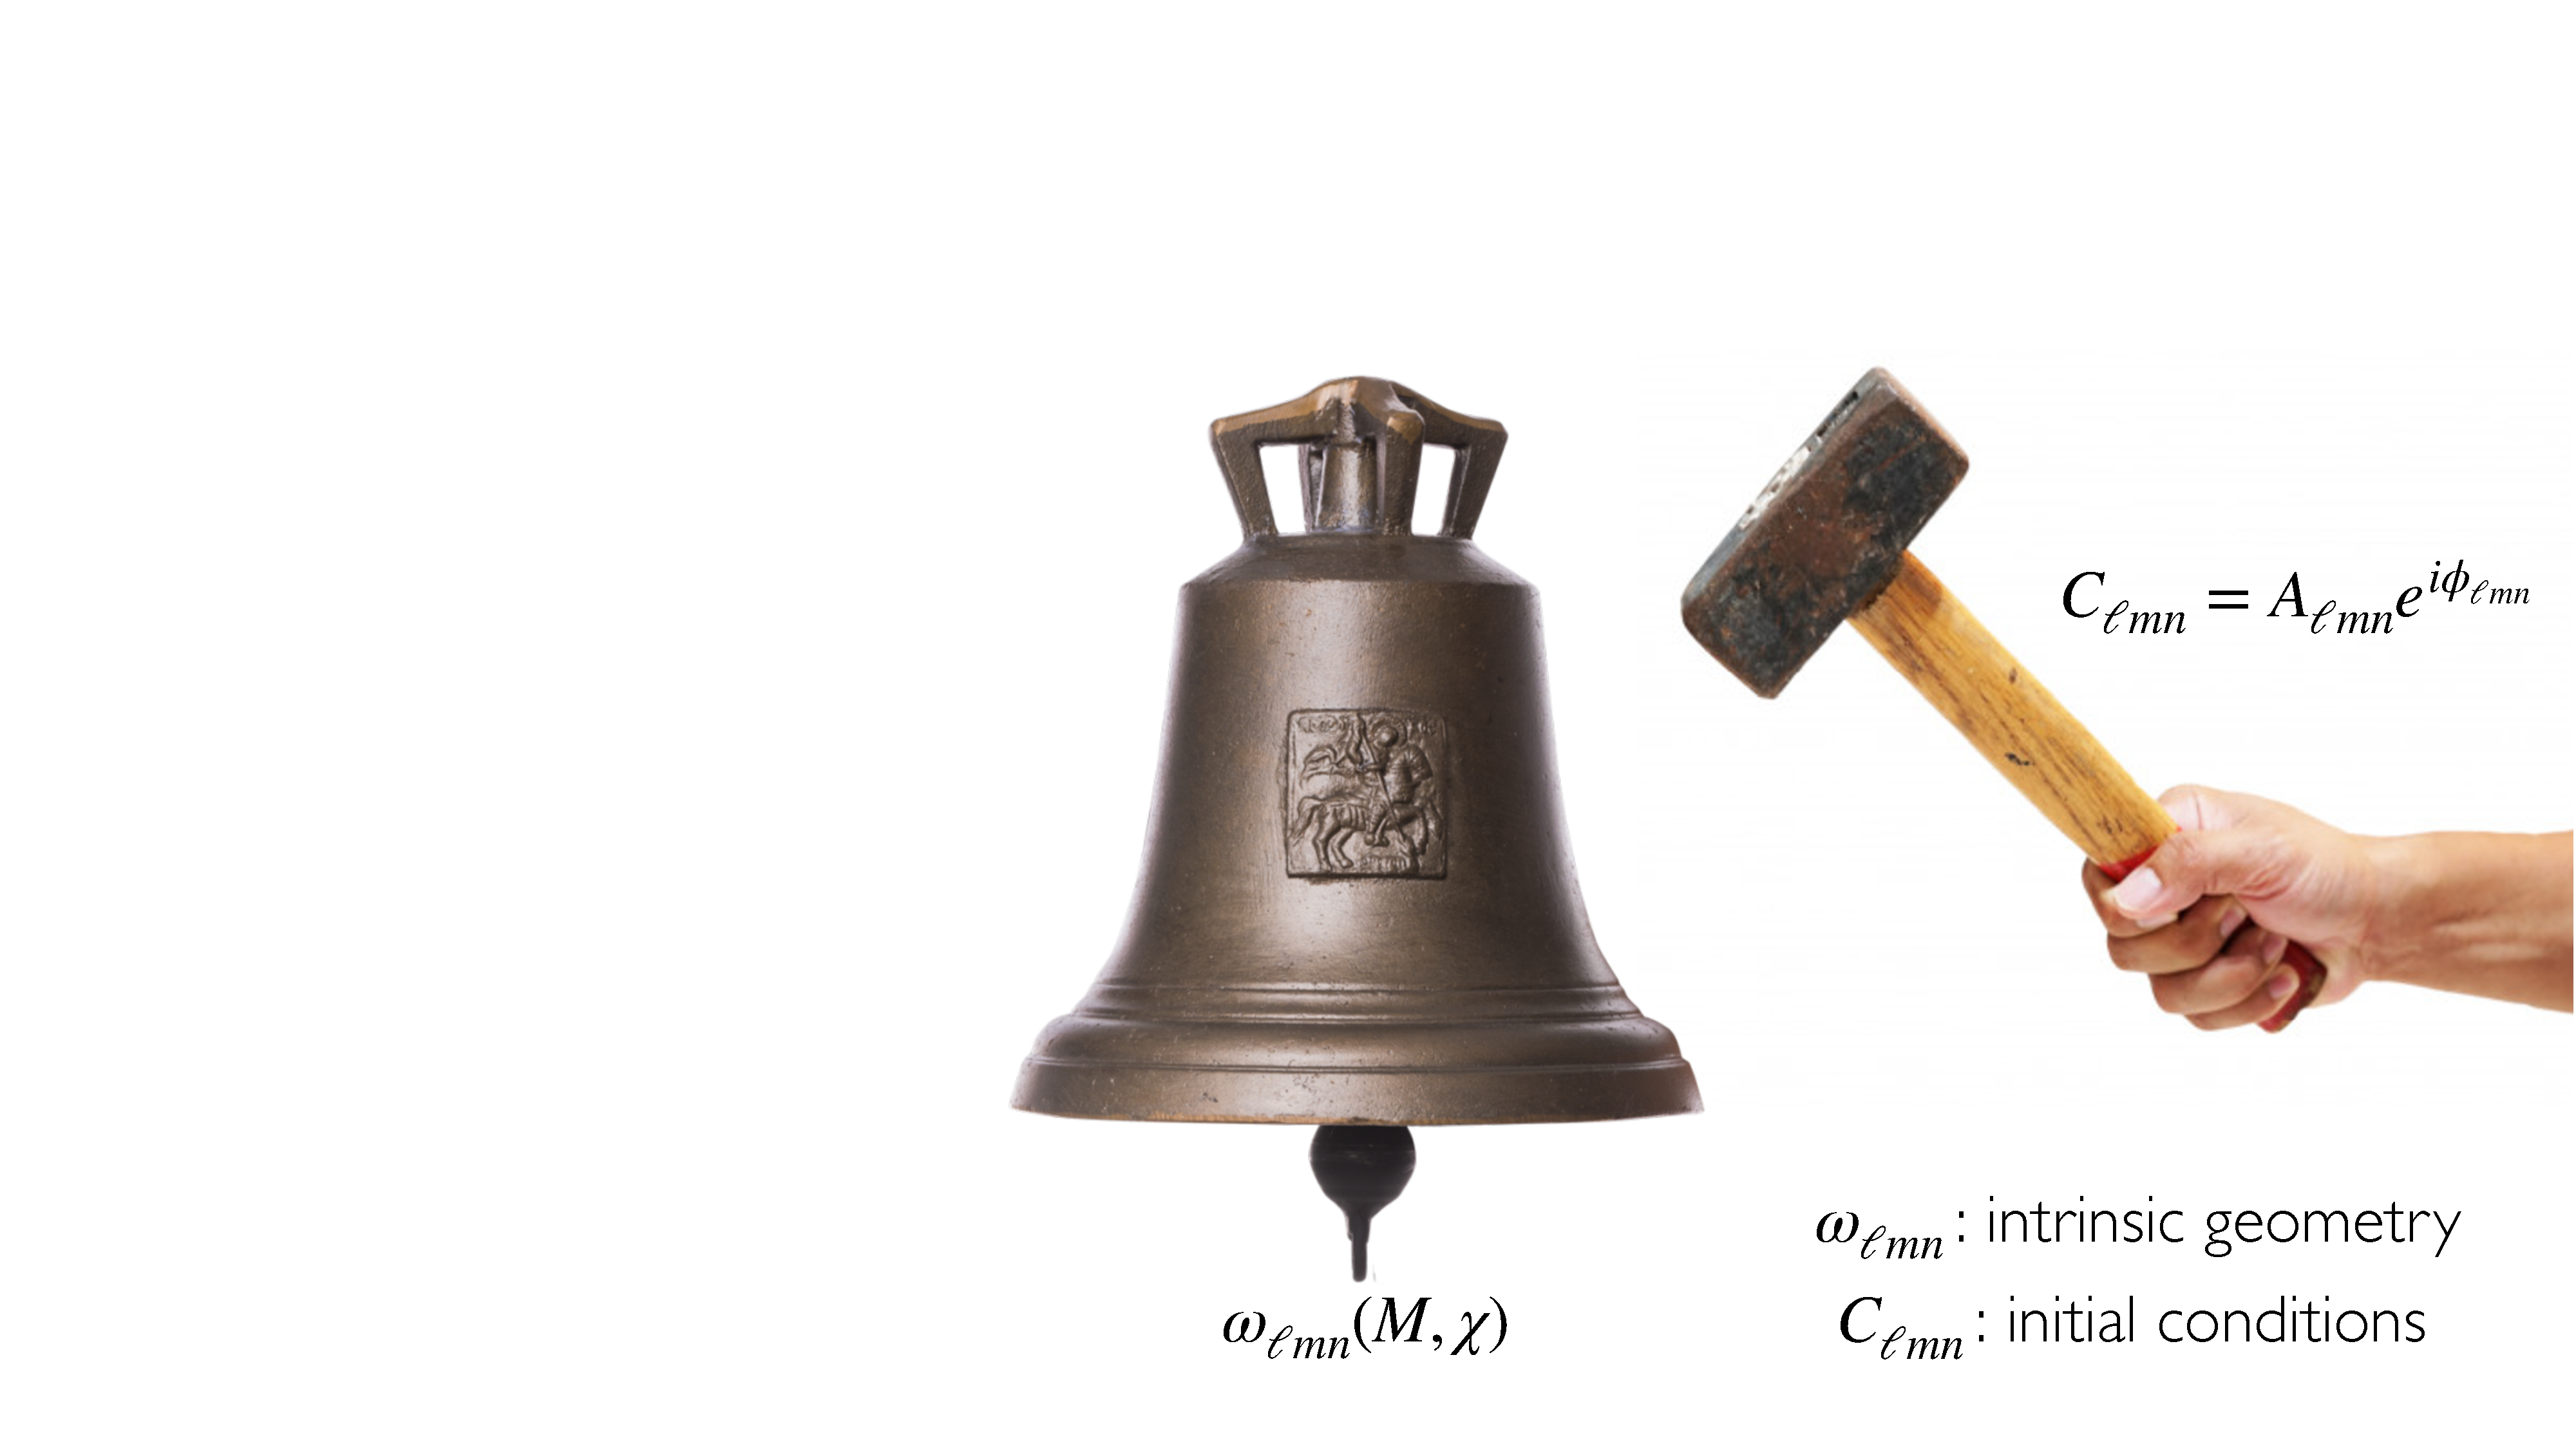
\includegraphics[width=0.5\columnwidth]{bell}
\caption{
A perturbed BH rings just like a struck bell.
The frequency $\omega_{\ell m n}$ and damping rate (pitch and duration) encode information about the intrinsic geometry of the object: mass and spin for a Kerr BH, shape and material for a bell.
The complex amplitudes $C_{\ell m n} = A_{\ell m n} e^{i\phi_{\ell m n}}$, on the other hand, carry information about the origin of the perturbation.
(\emph{Image source:} bell \cite{bell}, hammer \cite{hammer}.)
}
\label{fig:bell}
\end{figure}

Each QNM has a frequency $\omega_{\ell m n}$ and a damping time $\tau_{\ell m n}$, where $n$ is the overtone index and $(\ell,m)$ are indices of spin-weighted angular harmonics that describe the angular structure of the mode.
The overtone index $n$ orders the modes with a given $(\ell,m)$ by increasing damping rate, so that $n=0$ denotes the longest-lived (``fundamental'') mode.
Unlike elsewhere in physics, a higher $n$ does not imply a higher frequency $\omega_n$; rather, the opposite is generally true.

Our analysis targets the fundamental and overtones of the $\ell=m=2$ spin-weighted spherical harmonic of the strain, as this is the only angular harmonic expected to be relevant for GW150914 \cite{Abbott:2016apu,Abbott:2016wiq,Carullo:2019flw}.
We drop the $\ell$ and $m$ indices, and write the $\ell=m=2$ mode of the ringdown strain ($h=h_+ - i h_\times$) as a sum of damped sinusoids~\cite{Vishveshwara1970b,Press1971,Teukolsky,ChandraDetweiler1975},
\beq\label{eq:qnm}
  h_{22}^{N}(t) = \sum\limits_{n=0}^{N} A_n \exp\left[-i \left(\omega_n t + \phi_n\right) - t/\tau_n\right] ,
\eeq
for times $t$ greater than some start time $t_0$, where $\Delta t = t-t_0$.
$N$ is the index of the highest overtone included in the model, which for us will always be $N\leq 2$.
For a Kerr BH, all the $\omega_n$'s and  $\tau_n$'s are implicit functions of the remnant mass and spin magnitude ($\mf,\, \chif$), and can be computed from perturbation theory \cite{Leaver1985,Berti2009,BertiWebsite}.
The amplitudes $A_n$ and phases $\phi_n$ cannot be computed within perturbation theory, so we treat them as free parameters (\fig{bell}).

\begin{figure}[bt]
\centering
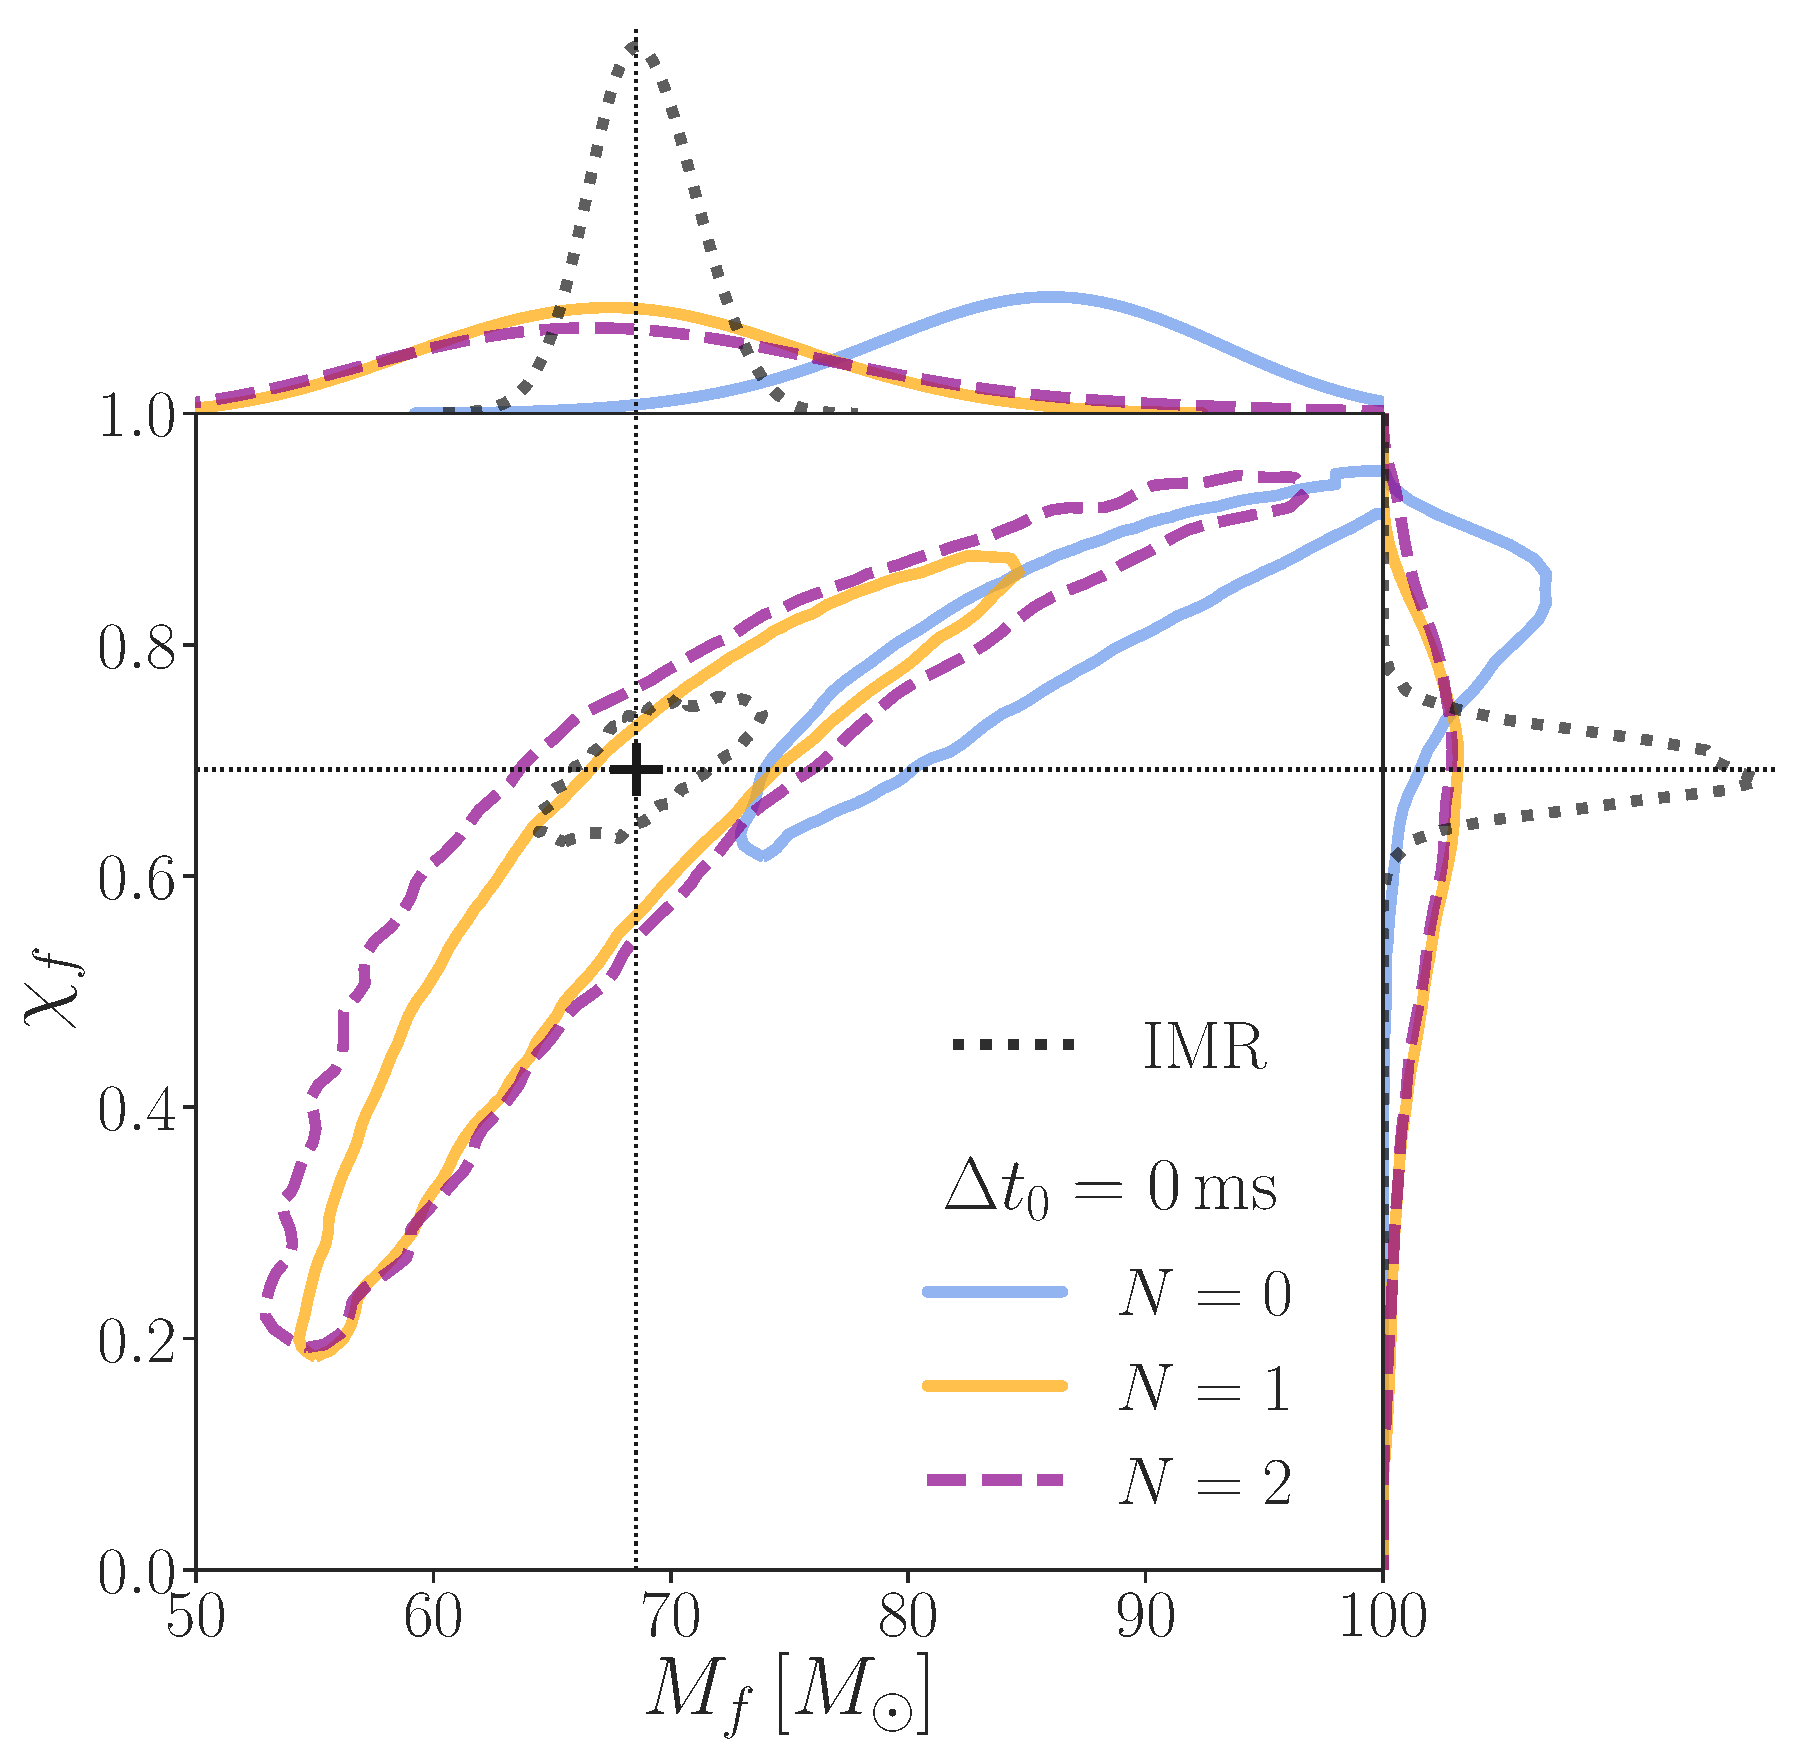
\includegraphics[width=0.66\columnwidth,clip=true]{contours_gw150914_n}
\caption{
    Contours represent 90\%-credible regions on the remnant mass ($\mf$) and dimensionless spin magnitude ($\chi_f$), obtained from the analysis of the  GW150914 ringdown starting at peak strain amplitude ($\Delta t_0 = t_0 - \tpeak = 0$).
    Color encodes the number of overtones $N$ in the model: 0 (solid blue), 1 (solid yellow), 2 (dashed purple)
    The dotted black contour is obtained from the full IMR waveform, assuming GR; the crosshairs mark the peak of this distribution ($\mf = 68.5 M_\odot$, $\chi_f=0.69$).
    The top and right panels show marginal posteriors for $\mf$ and $\chif$ respectively.
    This is Fig.~1 in \cite{Isi:2019aib}.
}
\label{fig:contours_n}
\end{figure}

We carry out a Bayesian analysis of LIGO Hanford and LIGO Livingston data for GW150914~\cite{gw150914,gwtc1:2018,gwosc}.
For a choice of $N$ and start time $t_0$, we compute the joint posterior probability over $\mf$, $\chi_f$, $A_n$ and $\phi_n$.
We first do so assuming a Kerr spectrum, but then relax the $N=1$ model to test the no-hair theorem: in this non-GR model, we write 
\beq
\omega_1=2\pi f^{\rm (GR)}_1\left(1+\delta f_1\right),
\eeq
\beq
\tau_1 = \tau^{\rm (GR)}_1\left(1+\delta\tau_1\right),
\eeq
with $\delta f_1$ and $\delta\tau_1$ fractional deviations away from the Kerr values $f^{\rm (GR)}_1$ and $\tau^{\rm (GR)}_1$ for any given $\mf$ and $\chif$.
In all cases, we parametrize start times via $\Delta t_0 = t_0 - \tpeak$, where $\tpeak = \tevent$ GPS refers to the signal peak at the LIGO Hanford detector \cite{gw150914_pe,gw150914_tgr}.
We define the likelihood in the time domain in order to explicitly exclude all data before $t_0$.
See the Supplement to \cite{Isi:2019aib} for details.

We compare our ringdown-only measurements to the expectation from the full inspiral-merger-ringdown (IMR) signal.
We use fitting formulas based on numerical relativity~\cite{Varma:2018aht,Blackman:2017pcm} to predict the remnant parameters from publicly-available posterior samples on the binary parameters \cite{gwtc1:2018,GWOSC:GWTC}.

\section{Results}

\fig{contours_n} shows the 90\%-credible regions for $\mf$ and $\chif$, obtained assuming a Kerr spectrum ($\delta f_n = \delta \tau_n=0$) by analyzing data starting at $\tpeak$ with different numbers of overtones ($N=0,1,2$) in the ringdown template of \eq{qnm}.
Under GR, the ringdown and IMR measurements should agree.
As expected for $\delta t_0 = 0$, this is only the case for the overtone results ($N \geq 1$), and not for the fundamental alone.
Adding a second overtone ($N=2$) does not improve agreement with IMR, which is expected given the network SNR of GW150914 \cite{Giesler:2019uxc}.

\begin{figure}[bt]
\centering
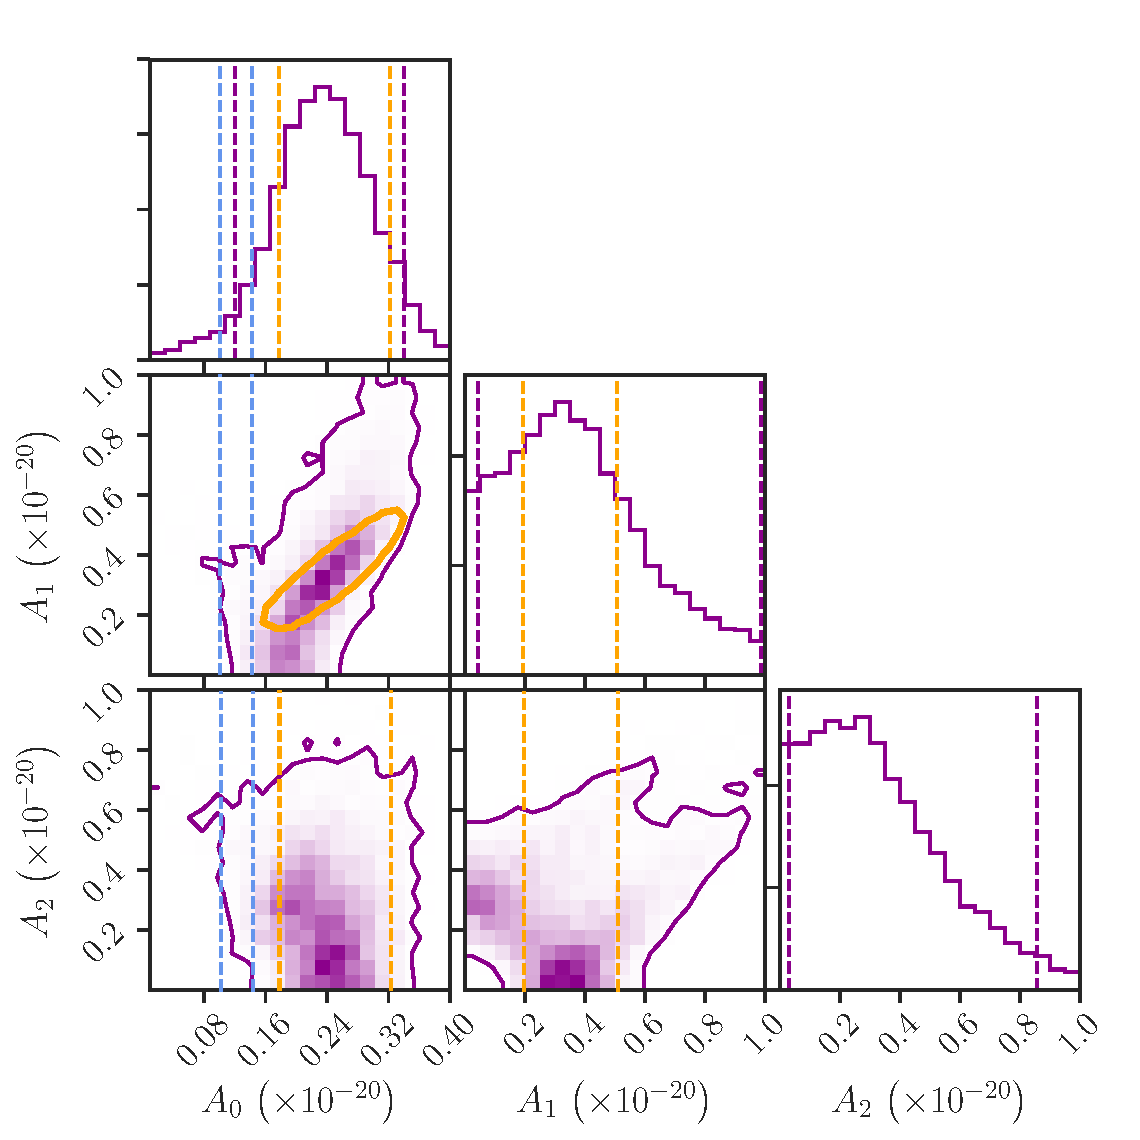
\includegraphics[width=0.66\columnwidth,clip=true]{corner_gw150914_allamps_n0}
\caption{
Measured QNM amplitudes for ringdown analyses with different number of overtones $N$, starting at peak strain:
the joint posterior for $A_0$, $A_1$ and $A_2$ recovered by the $N=2$ model (purple);
the 90\%-credible measurement of $A_0$ and $A_1$ obtained with $N=1$ (yellow); and the same for $A_0$ obtained with $N=0$ (blue).
Solid curves and vertical dashed lines enclose 90\% of the probability mass.
Values have been rescaled by a constant to correspond to the strain measured by the LIGO Hanford detector.
This is Fig.~2 in \cite{Isi:2019aib}.
}
\label{fig:allamps}
\end{figure}

The fact that the analysis is unable to unequivocally identify the second overtone in the data is reflected in the amplitude posteriors of \fig{allamps}.
The $N=2$ result supports a range of values for $A_1$ and $A_2$, but excludes $A_1=A_2=0$ with 90\% credibility (bottom center in \fig{allamps}).
The joint posterior distribution on $A_1$ and $A_2$ tends to favor the first overtone at the expense of the second, favoring a value of $A_1$ in agreement with the $N=1$ posterior (yellow traces in \fig{allamps}).
Assuming $N=1$, $A_1=0$ is disfavored at {$3.6\sigma$}; assuming $N=2$, $A_1=A_2=0$ is disfavored with 90\% credibility.

We next compare measurements carried out with overtones at the peak to those without overtones after the peak.
\fig{contours_t0} shows 90\%-credible regions for the remnant mass and spin magnitude obtained with $N=0$ at different times after $\tpeak$ ({$\Delta t_0 \in [1,\,3,\,5]\,\mathrm{ms}$}).
As the overtones die out, the fundamental mode becomes a better model for the signal, and we find that the $N=0$ contour coincides with the IMR measurement ${\sim}3\,$ms after the peak, in agreement with \cite{gw150914_tgr}.

\begin{figure}[bt]
\centering
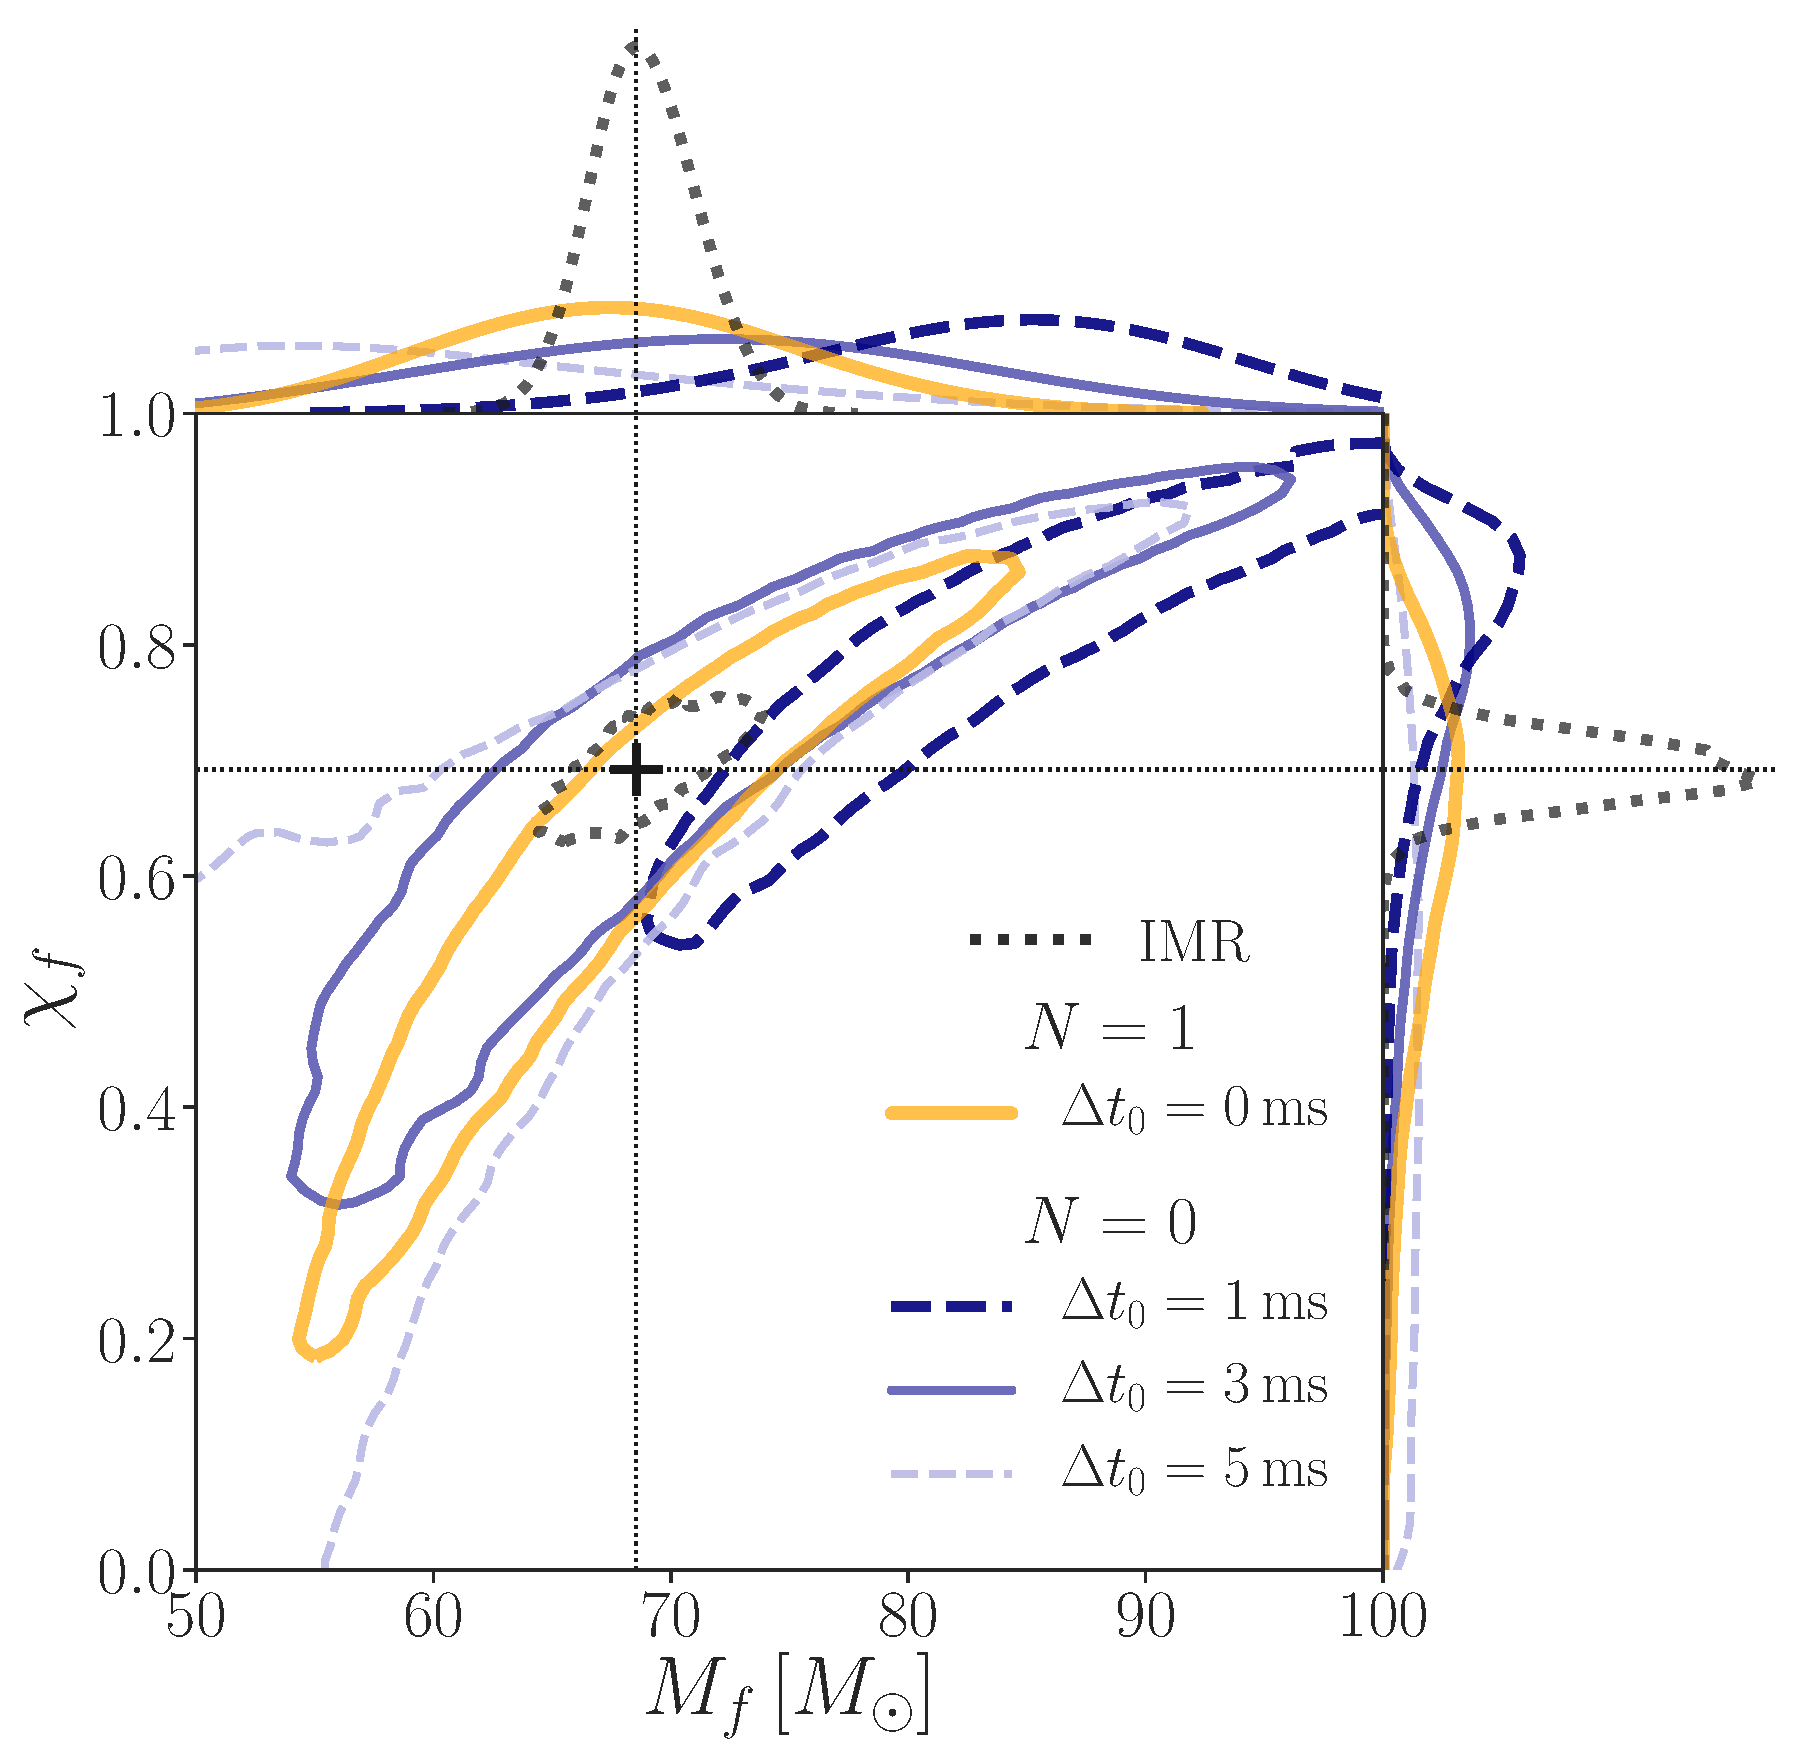
\includegraphics[width=0.66\columnwidth,clip=true]{contours_gw150914_t0}
\caption{
    Contours represent 90\%-credible regions on the remnant mass ($\mf$) and dimensionless spin magnitude ($\chi_f$), obtained from the analysis of the  GW150914 ringdown with $N=0$ at different times after the peak (blue), compared to $N=1$ at the peak.
    The dotted black contour is obtained from the full IMR waveform, assuming GR; the crosshairs mark the peak of this distribution ($\mf = 68.5 M_\odot$, $\chi_f=0.69$).
    The top and right panels show marginal posteriors for $\mf$ and $\chif$ respectively.
    Around $\Delta t_0 = 3\, \mathrm{ms}$, the overtones have become unmeasurable and only the fundamental mode remains; consequently, at that time, the $N=0$ result starts being consistent with both the full IMR waveform and the $N\geq 1$ models at the peak, in agreement with GR.
    This is Fig.~3 in \cite{Isi:2019aib}.
}
\label{fig:contours_t0}
\end{figure}

Finally, we allow the first-overtone frequency and damping time to float around the no-hair values in the $N=1$ model, starting the analysis at peak strain.
\fig{deltaf1} shows the resulting posterior over the $\delta f_1$ and $\delta\tau_1$.
With 68\% credibility, we measure $\delta f_1 = -0.05 \pm 0.2$, establishing agreement with the no-hair hypothesis ($\delta f_1 = 0$) at the 20\% level.
The damping time is largely unconstrained in the $-0.06 \lesssim \delta\tau_1 \lesssim 1$ range.


\section{Conclusion}
Making use of overtones, we extracted information about the GW150914 remnant using only postinspiral data, starting at the peak of the signal (\fig{contours_n}).
We found evidence of the fundamental mode plus at least one overtone (\fig{allamps}), and measured the remnant mass and spin in agreement with that the full waveform analysis.
This result is also consistent with the one obtained using solely the fundamental mode at a later time (\fig{contours_t0}).

The agreement between all measurements (IMR, $N=0$, $N\geq 1$) is evidence that, beginning as early as the signal peak, a far-away observer cannot distinguish the source from a linearly perturbed Kerr background, i.e., we do not observe nonlinearities in this regime.
The agreement between the IMR and postmerger estimates implies that the data conform to the full GR prediction, as in the IMR consistency test described in \cite{Ghosh:2016qgn,Ghosh:2017gfp}.

With the identification of multiple ringdown modes, we took a step toward the goal of black hole spectroscopy.
We constrained deviations away from the no-hair spectrum by allowing the overtone frequency and damping time to vary freely (\fig{deltaf1}).
This is equivalent to independently measuring the frequencies of the fundamental and first overtone, and establishing their consistency with the Kerr hypothesis.

Future overtone measurements could potentially allow us to identify BH mimickers, and probe the applicability of the no-hair theorem with high precision.
As the sensitivity of GW instruments improves, we will be able to leverage the increased quantity and quality of the detected signals to test the no-hair theorem in richer and more accurate ways.

\begin{figure}[bt]
\centering
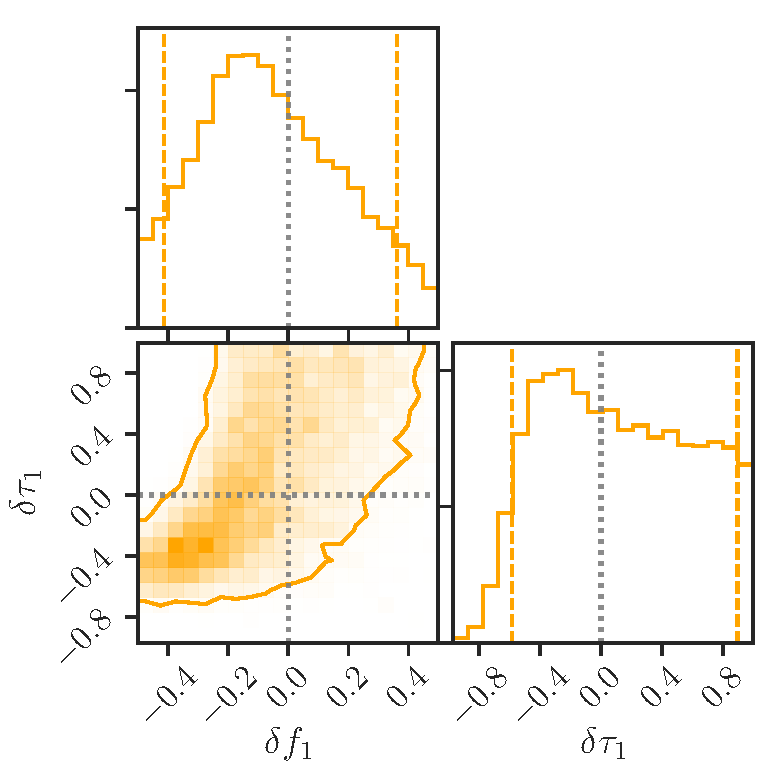
\includegraphics[width=0.66\columnwidth,clip=true]{delta_ftau1}
\caption{
Posterior distribution of the fractional deviations $\delta f_1$ and $\delta\tau_1$ away from the no-hair value $\delta f_1=\delta\tau_1=0$ (gray dotted lines), measured at peak strain with $N=1$.
The solid contour and dashed vertical lines enclose 90\% of the posterior probability.
Fixing $\delta f_1=\delta\tau_1 = 0$ recovers the $N=1$ analysis in Figs.~\ref{fig:contours_n} and \ref{fig:contours_t0}.
This is Fig.~4 in \cite{Isi:2019aib}.
}
\label{fig:deltaf1}
\end{figure}


\section*{Acknowledgements}
These Proceedings summarized \cite{Isi:2019aib}, as presented by M.I.~at the \emph{3rd World Summit on Exploring the Dark Side of the Universe} (Guadeloupe Islands, March 9-13 2020).
Besides M.I., the authors of this work were Matthew Giesler, Will M.~Farr, Mark A.~Scheel, and Saul A.~Teukolsky.
% NASA
M.I.\ is supported by NASA through the NASA Hubble Fellowship
grant No.\ HST-HF2-51410.001-A awarded by the Space Telescope
Science Institute, which is operated by the Association of Universities
for Research in Astronomy, Inc., for NASA, under contract NAS5-26555.
% LIGO
M.I.\ is a member of the LIGO Laboratory.
LIGO was constructed by the California Institute of Technology and
Massachusetts Institute of Technology with funding from the National
Science Foundation and operates under cooperative agreement PHY-0757058.
% Caltech
M.G.\ and M.S.\ are supported by the Sherman Fairchild Foundation and NSF
grants PHY-1708212 and PHY-1708213 at Caltech.
% Cornell
S.T.\ is supported in part by the Sherman Fairchild Foundation and by NSF Grants
PHY-1606654 and ACI-1713678 at Cornell.
% CCA
The Flatiron Institute is supported by the Simons Foundation.
% GWOSC
This research has made use of data, software and/or web tools obtained from the Gravitational Wave Open Science Center \cite{Vallisneri:2014vxa,gwosc}, a service of the LIGO Laboratory, the LIGO Scientific Collaboration and the Virgo Collaboration.

\bibliographystyle{JHEP} 
\bibliography{ligo,nr}

%\printindex

\end{document}
